\newpage 
 \clearpage 
 
Start Pre....
\hfill
\break
\newline
%============================================= Image ChokedFlow 
Fig. \ref{fig:ChokedFlow}
\input{../images/ChokedFlow.tex}
%============================================= Image FullFlowAntiBoundary 
Fig. \ref{fig:FullFlowAntiBoundary}
\input{../images/FullFlowAntiBoundary.tex}
%============================================= Image FullFlowSlice 
Fig. \ref{fig:FullFlowSlice}
\input{../images/FullFlowSlice.tex}
%============================================= Image FullFlow 
Fig. \ref{fig:FullFlow}
\input{../images/FullFlow.tex}
%============================================= Image SimpVectPlot 
Fig. \ref{fig:SimpVectPlot}
\input{../images/SimpVectPlot.tex}
%============================================= Image SimpleSequence 
Fig. \ref{fig:SimpleSequence}
\input{../images/SimpleSequence.tex}
%============================================= Image main_HSV2GradientSimp 
Fig. \ref{fig:main_HSV2GradientSimp}
\input{../images/main_HSV2GradientSimp.tex}
%============================================= Image GradientPlotLabelled 
Fig. \ref{fig:GradientPlotLabelled}
\input{../images/GradientPlotLabelled.tex}
%============================================= Image main_HSV2GradientLabelled 
Fig. \ref{fig:main_HSV2GradientLabelled}
\input{../images/main_HSV2GradientLabelled.tex}
%============================================= Image main_HSV2GradientSimp001 
Fig. \ref{fig:main_HSV2GradientSimp001}
\begin{figure}[H]
\centering
\includegraphics[width=1.70in]{../imgperm/main_HSV2GradientSimp001.png}
\captionof{figure}[Dobule Cone]{\textit{The setup for a simple demonstration. The particles in blue are arranged at the top and bottom of the starting point of the nozzle and aimed at the sloping sections.}}
\label{fig:main_HSV2GradientSimp001}
\end{figure}

%============================================= Image main_HSV2GradientSimp002 
Fig. \ref{fig:main_HSV2GradientSimp002}
\begin{figure}[H]
\centering
\includegraphics[width=1.70in]{../imgperm/main_HSV2GradientSimp002.png}
\captionof{figure}[Dobule Cone]{\textit{The setup for a simple demonstration. The particles in blue are arranged at the top and bottom of the starting point of the nozzle and aimed at the sloping sections.}}
\label{fig:main_HSV2GradientSimp002}
\end{figure}

%============================================= Image SimpleConfig 
Fig. \ref{fig:SimpleConfig}
\begin{figure}[H]
\centering
\includegraphics[width=2.97in]{../imgperm/SimpleConfig.png}
\captionof{figure}[Dobule Cone]{\textit{The setup for a simple demonstration. The particles in blue are arranged at the top and bottom of the starting point of the nozzle and aimed at the sloping sections.}}
\label{fig:SimpleConfig}
\end{figure}

%============================================= Image FullCDFlow 
Fig. \ref{fig:FullCDFlow}
\begin{figure}[H]
\centering
\includegraphics[width=2.97in]{../imgperm/FullCDFlow.png}
\captionof{figure}[Dobule Cone]{\textit{Flow thorugh a Converging-Diverging Nozzle HSV colorized to reflect the velocity angle.}}
\label{fig:FullCDFlow}
\end{figure}

%============================================= Image ParticleParticle 
Fig. \ref{fig:ParticleParticle}
% !TeX root = main.tex
\newpage
\clearpage
\section{Numerical methods and experimental setup } 

This section covers the theory of 3-d collisions between particles and particles with boundaries. These collisions change velocity so the final section discusses position update.

\subsection{Particle-Particle Collision Resolution} \label{pph}

Particle-particle collision is a vast subject, but as referenced earlier, these collisions are elastic. Although not very realistic, these collisions require only an equation for momentum exchange in three dimensions. Rounded cell collision detection processes collisions for each particle, not each particle pair. Therefore, each particle in a collision is resolved separately. This requires the same calculation twice. The particle being processed, and all particles against which it is being processed. The particle being processed is called the \textit{source particle} and the particle, or particles, against which it is being compared are called the \textit{target particles}.

The momentum equations use the dot product to project velocity onto the the line of impact, which is the tangent plane bisecting the line between the particle centers, as illustrated in Fig. \ref{fig:ParticleParticle}.
% !TeX root = main.tex
\newpage
\clearpage
\section{Numerical methods and experimental setup } 

This section covers the theory of 3-d collisions between particles and particles with boundaries. These collisions change velocity so the final section discusses position update.

\subsection{Particle-Particle Collision Resolution} \label{pph}

Particle-particle collision is a vast subject, but as referenced earlier, these collisions are elastic. Although not very realistic, these collisions require only an equation for momentum exchange in three dimensions. Rounded cell collision detection processes collisions for each particle, not each particle pair. Therefore, each particle in a collision is resolved separately. This requires the same calculation twice. The particle being processed, and all particles against which it is being processed. The particle being processed is called the \textit{source particle} and the particle, or particles, against which it is being compared are called the \textit{target particles}.

The momentum equations use the dot product to project velocity onto the the line of impact, which is the tangent plane bisecting the line between the particle centers, as illustrated in Fig. \ref{fig:ParticleParticle}.
% !TeX root = main.tex
\newpage
\clearpage
\section{Numerical methods and experimental setup } 

This section covers the theory of 3-d collisions between particles and particles with boundaries. These collisions change velocity so the final section discusses position update.

\subsection{Particle-Particle Collision Resolution} \label{pph}

Particle-particle collision is a vast subject, but as referenced earlier, these collisions are elastic. Although not very realistic, these collisions require only an equation for momentum exchange in three dimensions. Rounded cell collision detection processes collisions for each particle, not each particle pair. Therefore, each particle in a collision is resolved separately. This requires the same calculation twice. The particle being processed, and all particles against which it is being processed. The particle being processed is called the \textit{source particle} and the particle, or particles, against which it is being compared are called the \textit{target particles}.

The momentum equations use the dot product to project velocity onto the the line of impact, which is the tangent plane bisecting the line between the particle centers, as illustrated in Fig. \ref{fig:ParticleParticle}.
\input{../images/ParticleParticle.tex}

Equations (\ref{eqn:calcmom001}-\ref{eqn:calcmom004}) calculate parameters for the source particle.
\input{../equations/calcmom001.tex}
\input{../equations/calcmom002.tex}
\input{../equations/calcmom003.tex}
\input{../equations/calcmom004.tex}

Equations (\ref{eqn:calcmom005}-\ref{eqn:calcmom008}) calculate parameters for the target particle.
\input{../equations/calcmom005.tex}
\input{../equations/calcmom006.tex}
\input{../equations/calcmom007.tex}
\input{../equations/calcmom008.tex}

The velocity for the source particle is calculated as in \ref{eqn:calcmom009}.
\input{../equations/calcmom009.tex}

Collision resolution is processed in the compute pipeline. The \textit{potentially colliding set} is delivered to the compute kernel by the graphics pipeline. The code iterates over the eight corners of the \textit{axis aligned bounding box} (AABB) encasing the particle sphere, seeking other particle corners that occupy the same cell. The code traverses the length of the array which contains all of the particles in the cell. When a particle is found, it is registered in a duplicates array, since two or more particle corners can span the same cells. If it is not a duplicate the particle resolution is calculated.

Fig. \ref{fig:CalcMomentum} in section \ref{pbcrc}, shows this code in glsl a language that is 'built' for multidimensional calculus. For example, like templates in C++, variables types, like arrays and matrices, can be mulitplied, divided, added, subtracted, compared, etc, just like scalars. The GPU is also designed to process these type very efficiently.

The code for particle-particle collisions is detailed in the Appendix section \ref{ppcrc}

Equations (\ref{eqn:calcmom001}-\ref{eqn:calcmom004}) calculate parameters for the source particle.
\begin{equation}
 \begin{aligned}
 \hat{x}=\sfrac{\left(\vec{P_F}-\vec{P_T}\right)}{||\vec{x}||}\label{eqn:calcmom001} 
\end{aligned}
\end{equation}

\begin{equation}
 \begin{aligned}
 \vec{x_f}=\hat{x}\bullet\vec{v_f}\label{eqn:calcmom002} 
\end{aligned}
\end{equation}

\begin{equation}
 \begin{aligned}
 \vec{v_{fx}}=\hat{x}\left(\vec{x_f}\right)\label{eqn:calcmom003} 
\end{aligned}
\end{equation}

\begin{equation}
 \begin{aligned}
 \vec{v_{fy}}=\vec{x_f}-\vec{v_{fx}}\label{eqn:calcmom004} 
\end{aligned}
\end{equation}


Equations (\ref{eqn:calcmom005}-\ref{eqn:calcmom008}) calculate parameters for the target particle.
\begin{equation}
 \begin{aligned}
 \hat{x}=-\hat{x}\label{eqn:calcmom005} 
\end{aligned}
\end{equation}

\begin{equation}
 \begin{aligned}
 \vec{x_t}=\hat{x}\bullet\vec{v_t}\label{eqn:calcmom006} 
\end{aligned}
\end{equation}

\begin{equation}
 \begin{aligned}
 \vec{v_{tx}}=\hat{x}\left(\vec{x_t}\right)\label{eqn:calcmom007} 
\end{aligned}
\end{equation}

\begin{equation}
 \begin{aligned}
 \vec{v_{ty}}=\vec{x_f}-\vec{v_{tx}}\label{eqn:calcmom008} 
\end{aligned}
\end{equation}


The velocity for the source particle is calculated as in \ref{eqn:calcmom009}.
\begin{equation}
 \begin{aligned}
 \vec{V_f} = \vec{v_{fx}}\frac{(m_1-m_2)}{m_1+m_2}+\vec{v_{tx}}\frac{2(m_2)}{m_1+m_2}+\vec{v_{ty}}\label{eqn:calcmom009} 
\end{aligned}
\end{equation}


Collision resolution is processed in the compute pipeline. The \textit{potentially colliding set} is delivered to the compute kernel by the graphics pipeline. The code iterates over the eight corners of the \textit{axis aligned bounding box} (AABB) encasing the particle sphere, seeking other particle corners that occupy the same cell. The code traverses the length of the array which contains all of the particles in the cell. When a particle is found, it is registered in a duplicates array, since two or more particle corners can span the same cells. If it is not a duplicate the particle resolution is calculated.

Fig. \ref{fig:CalcMomentum} in section \ref{pbcrc}, shows this code in glsl a language that is 'built' for multidimensional calculus. For example, like templates in C++, variables types, like arrays and matrices, can be mulitplied, divided, added, subtracted, compared, etc, just like scalars. The GPU is also designed to process these type very efficiently.

The code for particle-particle collisions is detailed in the Appendix section \ref{ppcrc}

Equations (\ref{eqn:calcmom001}-\ref{eqn:calcmom004}) calculate parameters for the source particle.
\begin{equation}
 \begin{aligned}
 \hat{x}=\sfrac{\left(\vec{P_F}-\vec{P_T}\right)}{||\vec{x}||}\label{eqn:calcmom001} 
\end{aligned}
\end{equation}

\begin{equation}
 \begin{aligned}
 \vec{x_f}=\hat{x}\bullet\vec{v_f}\label{eqn:calcmom002} 
\end{aligned}
\end{equation}

\begin{equation}
 \begin{aligned}
 \vec{v_{fx}}=\hat{x}\left(\vec{x_f}\right)\label{eqn:calcmom003} 
\end{aligned}
\end{equation}

\begin{equation}
 \begin{aligned}
 \vec{v_{fy}}=\vec{x_f}-\vec{v_{fx}}\label{eqn:calcmom004} 
\end{aligned}
\end{equation}


Equations (\ref{eqn:calcmom005}-\ref{eqn:calcmom008}) calculate parameters for the target particle.
\begin{equation}
 \begin{aligned}
 \hat{x}=-\hat{x}\label{eqn:calcmom005} 
\end{aligned}
\end{equation}

\begin{equation}
 \begin{aligned}
 \vec{x_t}=\hat{x}\bullet\vec{v_t}\label{eqn:calcmom006} 
\end{aligned}
\end{equation}

\begin{equation}
 \begin{aligned}
 \vec{v_{tx}}=\hat{x}\left(\vec{x_t}\right)\label{eqn:calcmom007} 
\end{aligned}
\end{equation}

\begin{equation}
 \begin{aligned}
 \vec{v_{ty}}=\vec{x_f}-\vec{v_{tx}}\label{eqn:calcmom008} 
\end{aligned}
\end{equation}


The velocity for the source particle is calculated as in \ref{eqn:calcmom009}.
\begin{equation}
 \begin{aligned}
 \vec{V_f} = \vec{v_{fx}}\frac{(m_1-m_2)}{m_1+m_2}+\vec{v_{tx}}\frac{2(m_2)}{m_1+m_2}+\vec{v_{ty}}\label{eqn:calcmom009} 
\end{aligned}
\end{equation}


Collision resolution is processed in the compute pipeline. The \textit{potentially colliding set} is delivered to the compute kernel by the graphics pipeline. The code iterates over the eight corners of the \textit{axis aligned bounding box} (AABB) encasing the particle sphere, seeking other particle corners that occupy the same cell. The code traverses the length of the array which contains all of the particles in the cell. When a particle is found, it is registered in a duplicates array, since two or more particle corners can span the same cells. If it is not a duplicate the particle resolution is calculated.

Fig. \ref{fig:CalcMomentum} in section \ref{pbcrc}, shows this code in glsl a language that is 'built' for multidimensional calculus. For example, like templates in C++, variables types, like arrays and matrices, can be mulitplied, divided, added, subtracted, compared, etc, just like scalars. The GPU is also designed to process these type very efficiently.

The code for particle-particle collisions is detailed in the Appendix section \ref{ppcrc}
%============================================= Image GradientPlot 
Fig. \ref{fig:GradientPlot}
\begin{figure}[H]
\centering
\includegraphics[width=5.10in]{../imgperm/GradientPlot.png}
\captionof{figure}[Dobule Cone]{\textit{Gradient Field Appication.}}
\label{fig:GradientPlot}
\end{figure}

%============================================= Image main_HSV2Gradient 
Fig. \ref{fig:main_HSV2Gradient}
\begin{figure}[H]
\centering
\includegraphics[width=5.10in]{../imgperm/main_HSV2Gradient.png}
\captionof{figure}[Dobule Cone]{\textit{Main Evaluation Application.}}
\label{fig:main_HSV2Gradient}
\end{figure}

%============================================= Image InventortCDN 
Fig. \ref{fig:InventortCDN}
\begin{figure}[H]
\centering
\includegraphics[width=5.10in]{../images/InventortCDN.png}
\captionof{figure}[Dobule Cone]{\textit{Actual Converging-Diverging Nozzel design.}}
\label{fig:InventortCDN}
\end{figure}

%============================================= Image InventortCDNDWG 
Fig. \ref{fig:InventortCDNDWG}
\begin{figure}[H]
\centering
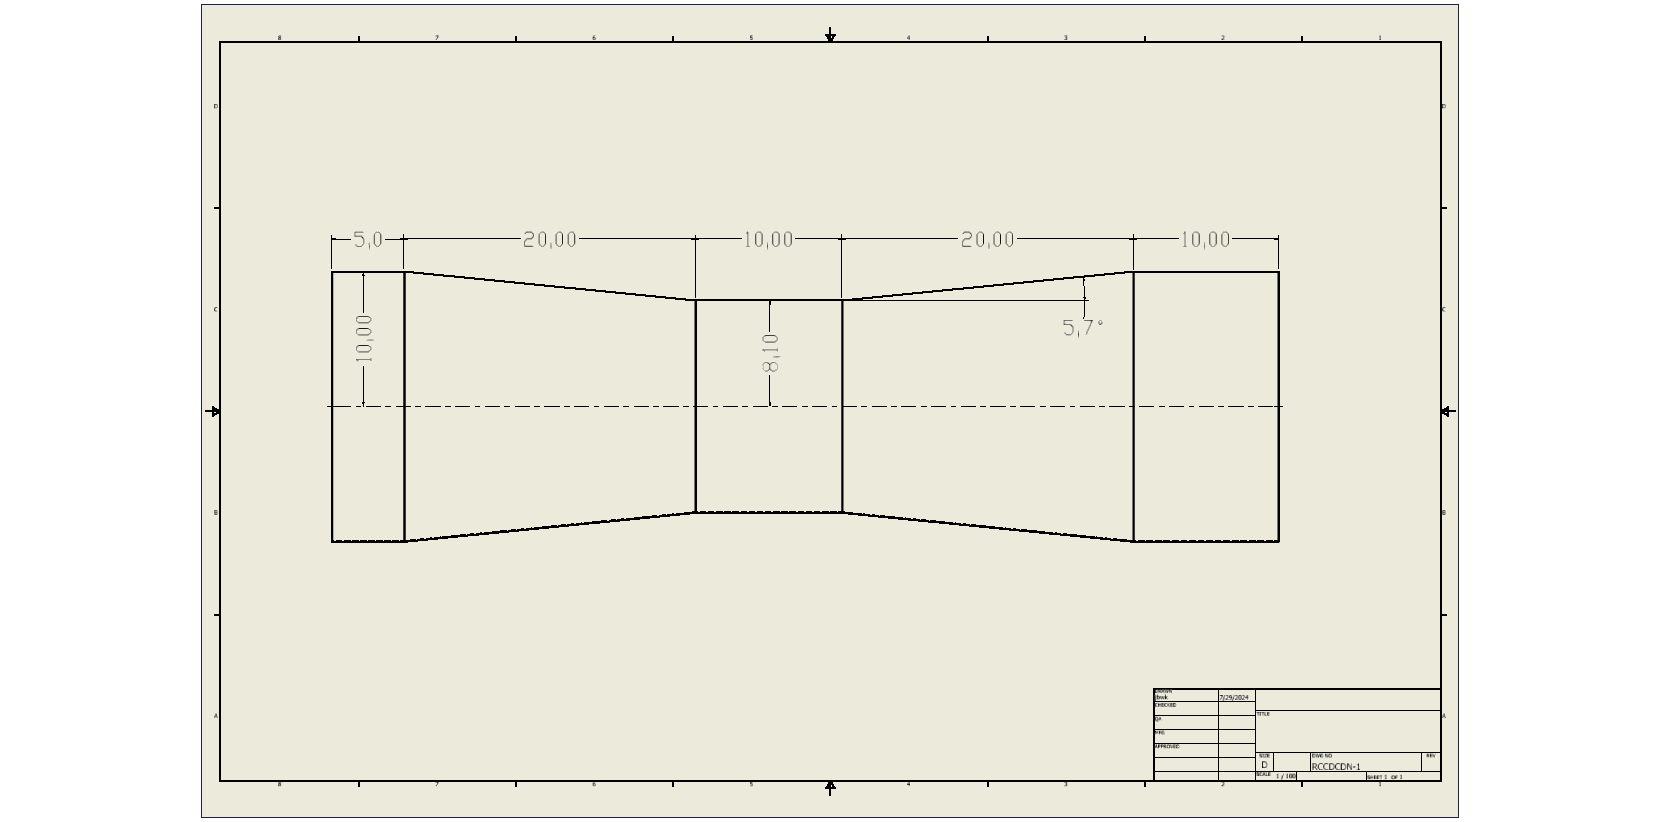
\includegraphics[width=6.80in]{../images/InventortCDNDWG.png}
\captionof{figure}[Dobule Cone]{\textit{Converging-Diverging Nozzel design specifications.}}
\label{fig:InventortCDNDWG}
\end{figure}

%============================================= Image Perf_gan2016 
Fig. \ref{fig:Perf_gan2016}
\begin{multiFigure}
\centering
{
\addFigure{0.40}{../images/Perf_gan2016_01.png} \qquad
\addFigure{0.40}{../imgperm/Perf_gan2016_02.png} \qquad
}
\captionof{figure}[Perfornamce Data Gan]{\textit{Performance plots from \textit{A GPU-based DEM approach for modelling of particulate systems.} \citep{gan2016}.}}
\label{fig:Perf_gan2016}
\end{multiFigure}

%============================================= Image olej 
Fig. \ref{fig:olej}
\begin{figure}[H]
\centering
\includegraphics[width=3.40in]{../images/DoubleCone.png}
\captionof{figure}[Dobule Cone]{\textit{Double-cone Flow field schematic (after Olejniczak,Candler \& Hornung \citep{olejniczak1997}).}}
\label{fig:olej}
\end{figure}

%============================================= Equation haus
\begin{verbatim}{Equation = haus}\end{verbatim}
(\ref{eqn:haus})
\begin{equation}
 \begin{aligned}
 haus\left( A,B \right) = {max \atop {a \in A }} {min \atop {b \in B}} \left| a-b \right|\label{eqn:haus} 
\end{aligned}
\end{equation}

%============================================= Equation span
\begin{verbatim}{Equation = span}\end{verbatim}
(\ref{eqn:span})
\begin{equation}
 \begin{aligned}
 span\left( A,B \right) = {max \atop {a \in A }} {max \atop {b \in B}} \left| a-b \right|\label{eqn:span} 
\end{aligned}
\end{equation}

%============================================= Equation pd
\begin{verbatim}{Equation = pd}\end{verbatim}
(\ref{eqn:pd})
\begin{equation}
 \begin{aligned}
 pd\left( A,B \right) = minimum \left\Vert v \right\Vert such \quad  that\quad  {min \atop {a \in A }} {min \atop {b \in B}} \left| \boldsymbol{a-b+v} \right|\geq0\label{eqn:pd} 
\end{aligned}
\end{equation}

%============================================= Equation gpd
\begin{verbatim}{Equation = gpd}\end{verbatim}
(\ref{eqn:gpd})
\begin{equation}
 \begin{aligned}
 gpd\left( A,B \right) = minimum \left\Vert \boldsymbol{M} \right\Vert_d such \quad  that\quad  {min \atop {a \in A }} {min \atop {b \in B}} \left| \boldsymbol{a-Mb} \right|\geq0\label{eqn:gpd} 
\end{aligned}
\end{equation}

%============================================= Equation calcmom001
\begin{verbatim}{Equation = calcmom001}\end{verbatim}
(\ref{eqn:calcmom001})
\begin{equation}
 \begin{aligned}
 \hat{x}=\sfrac{\left(\vec{P_F}-\vec{P_T}\right)}{||\vec{x}||}\label{eqn:calcmom001} 
\end{aligned}
\end{equation}

%============================================= Equation calcmom002
\begin{verbatim}{Equation = calcmom002}\end{verbatim}
(\ref{eqn:calcmom002})
\begin{equation}
 \begin{aligned}
 \vec{x_f}=\hat{x}\bullet\vec{v_f}\label{eqn:calcmom002} 
\end{aligned}
\end{equation}

%============================================= Equation calcmom003
\begin{verbatim}{Equation = calcmom003}\end{verbatim}
(\ref{eqn:calcmom003})
\begin{equation}
 \begin{aligned}
 \vec{v_{fx}}=\hat{x}\left(\vec{x_f}\right)\label{eqn:calcmom003} 
\end{aligned}
\end{equation}

%============================================= Equation calcmom004
\begin{verbatim}{Equation = calcmom004}\end{verbatim}
(\ref{eqn:calcmom004})
\begin{equation}
 \begin{aligned}
 \vec{v_{fy}}=\vec{x_f}-\vec{v_{fx}}\label{eqn:calcmom004} 
\end{aligned}
\end{equation}

%============================================= Equation calcmom005
\begin{verbatim}{Equation = calcmom005}\end{verbatim}
(\ref{eqn:calcmom005})
\begin{equation}
 \begin{aligned}
 \hat{x}=-\hat{x}\label{eqn:calcmom005} 
\end{aligned}
\end{equation}

%============================================= Equation calcmom006
\begin{verbatim}{Equation = calcmom006}\end{verbatim}
(\ref{eqn:calcmom006})
\begin{equation}
 \begin{aligned}
 \vec{x_t}=\hat{x}\bullet\vec{v_t}\label{eqn:calcmom006} 
\end{aligned}
\end{equation}

%============================================= Equation calcmom007
\begin{verbatim}{Equation = calcmom007}\end{verbatim}
(\ref{eqn:calcmom007})
\begin{equation}
 \begin{aligned}
 \vec{v_{tx}}=\hat{x}\left(\vec{x_t}\right)\label{eqn:calcmom007} 
\end{aligned}
\end{equation}

%============================================= Equation calcmom008
\begin{verbatim}{Equation = calcmom008}\end{verbatim}
(\ref{eqn:calcmom008})
\begin{equation}
 \begin{aligned}
 \vec{v_{ty}}=\vec{x_f}-\vec{v_{tx}}\label{eqn:calcmom008} 
\end{aligned}
\end{equation}

%============================================= Equation calcmom009
\begin{verbatim}{Equation = calcmom009}\end{verbatim}
(\ref{eqn:calcmom009})
\begin{equation}
 \begin{aligned}
 \vec{V_f} = \vec{v_{fx}}\frac{(m_1-m_2)}{m_1+m_2}+\vec{v_{tx}}\frac{2(m_2)}{m_1+m_2}+\vec{v_{ty}}\label{eqn:calcmom009} 
\end{aligned}
\end{equation}

%============================================= Equation bound001
\begin{verbatim}{Equation = bound001}\end{verbatim}
(\ref{eqn:bound001})
\begin{equation}
 \begin{aligned}
 \hat{N}=\frac{\left(\vec{P_a}-\vec{P_b}\right)\otimes\left(\vec{P_a}-\vec{P_c}\right)}{||\vec{N}||}\label{eqn:bound001} 
\end{aligned}
\end{equation}

%============================================= Equation bound002
\begin{verbatim}{Equation = bound002}\end{verbatim}
(\ref{eqn:bound002})
\begin{equation}
 \begin{aligned}
 \vec{V_{out}} = \vec{V_{in}} - 2.0(\vec{V_{in}}\bullet\hat{N})\hat{N}\label{eqn:bound002} 
\end{aligned}
\end{equation}




%============================================= Image ChokedFlow 
Fig. \ref{fig:ChokedFlow}
\input{../images/ChokedFlow.tex}
%============================================= Image FullFlowAntiBoundary 
Fig. \ref{fig:FullFlowAntiBoundary}
\input{../images/FullFlowAntiBoundary.tex}
%============================================= Image FullFlowSlice 
Fig. \ref{fig:FullFlowSlice}
\input{../images/FullFlowSlice.tex}
%============================================= Image FullFlow 
Fig. \ref{fig:FullFlow}
\input{../images/FullFlow.tex}
%============================================= Image SimpVectPlot 
Fig. \ref{fig:SimpVectPlot}
\input{../images/SimpVectPlot.tex}
%============================================= Image SimpleSequence 
Fig. \ref{fig:SimpleSequence}
\input{../images/SimpleSequence.tex}
%============================================= Image main_HSV2GradientSimp 
Fig. \ref{fig:main_HSV2GradientSimp}
\input{../images/main_HSV2GradientSimp.tex}
%============================================= Image GradientPlotLabelled 
Fig. \ref{fig:GradientPlotLabelled}
\input{../images/GradientPlotLabelled.tex}
%============================================= Image main_HSV2GradientLabelled 
Fig. \ref{fig:main_HSV2GradientLabelled}
\input{../images/main_HSV2GradientLabelled.tex}
%============================================= Image main_HSV2GradientSimp001 
Fig. \ref{fig:main_HSV2GradientSimp001}
\begin{figure}[H]
\centering
\includegraphics[width=1.70in]{../imgperm/main_HSV2GradientSimp001.png}
\captionof{figure}[Dobule Cone]{\textit{The setup for a simple demonstration. The particles in blue are arranged at the top and bottom of the starting point of the nozzle and aimed at the sloping sections.}}
\label{fig:main_HSV2GradientSimp001}
\end{figure}

%============================================= Image main_HSV2GradientSimp002 
Fig. \ref{fig:main_HSV2GradientSimp002}
\begin{figure}[H]
\centering
\includegraphics[width=1.70in]{../imgperm/main_HSV2GradientSimp002.png}
\captionof{figure}[Dobule Cone]{\textit{The setup for a simple demonstration. The particles in blue are arranged at the top and bottom of the starting point of the nozzle and aimed at the sloping sections.}}
\label{fig:main_HSV2GradientSimp002}
\end{figure}

%============================================= Image SimpleConfig 
Fig. \ref{fig:SimpleConfig}
\begin{figure}[H]
\centering
\includegraphics[width=2.97in]{../imgperm/SimpleConfig.png}
\captionof{figure}[Dobule Cone]{\textit{The setup for a simple demonstration. The particles in blue are arranged at the top and bottom of the starting point of the nozzle and aimed at the sloping sections.}}
\label{fig:SimpleConfig}
\end{figure}

%============================================= Image FullCDFlow 
Fig. \ref{fig:FullCDFlow}
\begin{figure}[H]
\centering
\includegraphics[width=2.97in]{../imgperm/FullCDFlow.png}
\captionof{figure}[Dobule Cone]{\textit{Flow thorugh a Converging-Diverging Nozzle HSV colorized to reflect the velocity angle.}}
\label{fig:FullCDFlow}
\end{figure}

%============================================= Image ParticleParticle 
Fig. \ref{fig:ParticleParticle}
% !TeX root = main.tex
\newpage
\clearpage
\section{Numerical methods and experimental setup } 

This section covers the theory of 3-d collisions between particles and particles with boundaries. These collisions change velocity so the final section discusses position update.

\subsection{Particle-Particle Collision Resolution} \label{pph}

Particle-particle collision is a vast subject, but as referenced earlier, these collisions are elastic. Although not very realistic, these collisions require only an equation for momentum exchange in three dimensions. Rounded cell collision detection processes collisions for each particle, not each particle pair. Therefore, each particle in a collision is resolved separately. This requires the same calculation twice. The particle being processed, and all particles against which it is being processed. The particle being processed is called the \textit{source particle} and the particle, or particles, against which it is being compared are called the \textit{target particles}.

The momentum equations use the dot product to project velocity onto the the line of impact, which is the tangent plane bisecting the line between the particle centers, as illustrated in Fig. \ref{fig:ParticleParticle}.
% !TeX root = main.tex
\newpage
\clearpage
\section{Numerical methods and experimental setup } 

This section covers the theory of 3-d collisions between particles and particles with boundaries. These collisions change velocity so the final section discusses position update.

\subsection{Particle-Particle Collision Resolution} \label{pph}

Particle-particle collision is a vast subject, but as referenced earlier, these collisions are elastic. Although not very realistic, these collisions require only an equation for momentum exchange in three dimensions. Rounded cell collision detection processes collisions for each particle, not each particle pair. Therefore, each particle in a collision is resolved separately. This requires the same calculation twice. The particle being processed, and all particles against which it is being processed. The particle being processed is called the \textit{source particle} and the particle, or particles, against which it is being compared are called the \textit{target particles}.

The momentum equations use the dot product to project velocity onto the the line of impact, which is the tangent plane bisecting the line between the particle centers, as illustrated in Fig. \ref{fig:ParticleParticle}.
% !TeX root = main.tex
\newpage
\clearpage
\section{Numerical methods and experimental setup } 

This section covers the theory of 3-d collisions between particles and particles with boundaries. These collisions change velocity so the final section discusses position update.

\subsection{Particle-Particle Collision Resolution} \label{pph}

Particle-particle collision is a vast subject, but as referenced earlier, these collisions are elastic. Although not very realistic, these collisions require only an equation for momentum exchange in three dimensions. Rounded cell collision detection processes collisions for each particle, not each particle pair. Therefore, each particle in a collision is resolved separately. This requires the same calculation twice. The particle being processed, and all particles against which it is being processed. The particle being processed is called the \textit{source particle} and the particle, or particles, against which it is being compared are called the \textit{target particles}.

The momentum equations use the dot product to project velocity onto the the line of impact, which is the tangent plane bisecting the line between the particle centers, as illustrated in Fig. \ref{fig:ParticleParticle}.
\input{../images/ParticleParticle.tex}

Equations (\ref{eqn:calcmom001}-\ref{eqn:calcmom004}) calculate parameters for the source particle.
\input{../equations/calcmom001.tex}
\input{../equations/calcmom002.tex}
\input{../equations/calcmom003.tex}
\input{../equations/calcmom004.tex}

Equations (\ref{eqn:calcmom005}-\ref{eqn:calcmom008}) calculate parameters for the target particle.
\input{../equations/calcmom005.tex}
\input{../equations/calcmom006.tex}
\input{../equations/calcmom007.tex}
\input{../equations/calcmom008.tex}

The velocity for the source particle is calculated as in \ref{eqn:calcmom009}.
\input{../equations/calcmom009.tex}

Collision resolution is processed in the compute pipeline. The \textit{potentially colliding set} is delivered to the compute kernel by the graphics pipeline. The code iterates over the eight corners of the \textit{axis aligned bounding box} (AABB) encasing the particle sphere, seeking other particle corners that occupy the same cell. The code traverses the length of the array which contains all of the particles in the cell. When a particle is found, it is registered in a duplicates array, since two or more particle corners can span the same cells. If it is not a duplicate the particle resolution is calculated.

Fig. \ref{fig:CalcMomentum} in section \ref{pbcrc}, shows this code in glsl a language that is 'built' for multidimensional calculus. For example, like templates in C++, variables types, like arrays and matrices, can be mulitplied, divided, added, subtracted, compared, etc, just like scalars. The GPU is also designed to process these type very efficiently.

The code for particle-particle collisions is detailed in the Appendix section \ref{ppcrc}

Equations (\ref{eqn:calcmom001}-\ref{eqn:calcmom004}) calculate parameters for the source particle.
\begin{equation}
 \begin{aligned}
 \hat{x}=\sfrac{\left(\vec{P_F}-\vec{P_T}\right)}{||\vec{x}||}\label{eqn:calcmom001} 
\end{aligned}
\end{equation}

\begin{equation}
 \begin{aligned}
 \vec{x_f}=\hat{x}\bullet\vec{v_f}\label{eqn:calcmom002} 
\end{aligned}
\end{equation}

\begin{equation}
 \begin{aligned}
 \vec{v_{fx}}=\hat{x}\left(\vec{x_f}\right)\label{eqn:calcmom003} 
\end{aligned}
\end{equation}

\begin{equation}
 \begin{aligned}
 \vec{v_{fy}}=\vec{x_f}-\vec{v_{fx}}\label{eqn:calcmom004} 
\end{aligned}
\end{equation}


Equations (\ref{eqn:calcmom005}-\ref{eqn:calcmom008}) calculate parameters for the target particle.
\begin{equation}
 \begin{aligned}
 \hat{x}=-\hat{x}\label{eqn:calcmom005} 
\end{aligned}
\end{equation}

\begin{equation}
 \begin{aligned}
 \vec{x_t}=\hat{x}\bullet\vec{v_t}\label{eqn:calcmom006} 
\end{aligned}
\end{equation}

\begin{equation}
 \begin{aligned}
 \vec{v_{tx}}=\hat{x}\left(\vec{x_t}\right)\label{eqn:calcmom007} 
\end{aligned}
\end{equation}

\begin{equation}
 \begin{aligned}
 \vec{v_{ty}}=\vec{x_f}-\vec{v_{tx}}\label{eqn:calcmom008} 
\end{aligned}
\end{equation}


The velocity for the source particle is calculated as in \ref{eqn:calcmom009}.
\begin{equation}
 \begin{aligned}
 \vec{V_f} = \vec{v_{fx}}\frac{(m_1-m_2)}{m_1+m_2}+\vec{v_{tx}}\frac{2(m_2)}{m_1+m_2}+\vec{v_{ty}}\label{eqn:calcmom009} 
\end{aligned}
\end{equation}


Collision resolution is processed in the compute pipeline. The \textit{potentially colliding set} is delivered to the compute kernel by the graphics pipeline. The code iterates over the eight corners of the \textit{axis aligned bounding box} (AABB) encasing the particle sphere, seeking other particle corners that occupy the same cell. The code traverses the length of the array which contains all of the particles in the cell. When a particle is found, it is registered in a duplicates array, since two or more particle corners can span the same cells. If it is not a duplicate the particle resolution is calculated.

Fig. \ref{fig:CalcMomentum} in section \ref{pbcrc}, shows this code in glsl a language that is 'built' for multidimensional calculus. For example, like templates in C++, variables types, like arrays and matrices, can be mulitplied, divided, added, subtracted, compared, etc, just like scalars. The GPU is also designed to process these type very efficiently.

The code for particle-particle collisions is detailed in the Appendix section \ref{ppcrc}

Equations (\ref{eqn:calcmom001}-\ref{eqn:calcmom004}) calculate parameters for the source particle.
\begin{equation}
 \begin{aligned}
 \hat{x}=\sfrac{\left(\vec{P_F}-\vec{P_T}\right)}{||\vec{x}||}\label{eqn:calcmom001} 
\end{aligned}
\end{equation}

\begin{equation}
 \begin{aligned}
 \vec{x_f}=\hat{x}\bullet\vec{v_f}\label{eqn:calcmom002} 
\end{aligned}
\end{equation}

\begin{equation}
 \begin{aligned}
 \vec{v_{fx}}=\hat{x}\left(\vec{x_f}\right)\label{eqn:calcmom003} 
\end{aligned}
\end{equation}

\begin{equation}
 \begin{aligned}
 \vec{v_{fy}}=\vec{x_f}-\vec{v_{fx}}\label{eqn:calcmom004} 
\end{aligned}
\end{equation}


Equations (\ref{eqn:calcmom005}-\ref{eqn:calcmom008}) calculate parameters for the target particle.
\begin{equation}
 \begin{aligned}
 \hat{x}=-\hat{x}\label{eqn:calcmom005} 
\end{aligned}
\end{equation}

\begin{equation}
 \begin{aligned}
 \vec{x_t}=\hat{x}\bullet\vec{v_t}\label{eqn:calcmom006} 
\end{aligned}
\end{equation}

\begin{equation}
 \begin{aligned}
 \vec{v_{tx}}=\hat{x}\left(\vec{x_t}\right)\label{eqn:calcmom007} 
\end{aligned}
\end{equation}

\begin{equation}
 \begin{aligned}
 \vec{v_{ty}}=\vec{x_f}-\vec{v_{tx}}\label{eqn:calcmom008} 
\end{aligned}
\end{equation}


The velocity for the source particle is calculated as in \ref{eqn:calcmom009}.
\begin{equation}
 \begin{aligned}
 \vec{V_f} = \vec{v_{fx}}\frac{(m_1-m_2)}{m_1+m_2}+\vec{v_{tx}}\frac{2(m_2)}{m_1+m_2}+\vec{v_{ty}}\label{eqn:calcmom009} 
\end{aligned}
\end{equation}


Collision resolution is processed in the compute pipeline. The \textit{potentially colliding set} is delivered to the compute kernel by the graphics pipeline. The code iterates over the eight corners of the \textit{axis aligned bounding box} (AABB) encasing the particle sphere, seeking other particle corners that occupy the same cell. The code traverses the length of the array which contains all of the particles in the cell. When a particle is found, it is registered in a duplicates array, since two or more particle corners can span the same cells. If it is not a duplicate the particle resolution is calculated.

Fig. \ref{fig:CalcMomentum} in section \ref{pbcrc}, shows this code in glsl a language that is 'built' for multidimensional calculus. For example, like templates in C++, variables types, like arrays and matrices, can be mulitplied, divided, added, subtracted, compared, etc, just like scalars. The GPU is also designed to process these type very efficiently.

The code for particle-particle collisions is detailed in the Appendix section \ref{ppcrc}
%============================================= Image GradientPlot 
Fig. \ref{fig:GradientPlot}
\begin{figure}[H]
\centering
\includegraphics[width=5.10in]{../imgperm/GradientPlot.png}
\captionof{figure}[Dobule Cone]{\textit{Gradient Field Appication.}}
\label{fig:GradientPlot}
\end{figure}

%============================================= Image main_HSV2Gradient 
Fig. \ref{fig:main_HSV2Gradient}
\begin{figure}[H]
\centering
\includegraphics[width=5.10in]{../imgperm/main_HSV2Gradient.png}
\captionof{figure}[Dobule Cone]{\textit{Main Evaluation Application.}}
\label{fig:main_HSV2Gradient}
\end{figure}

%============================================= Image InventortCDN 
Fig. \ref{fig:InventortCDN}
\begin{figure}[H]
\centering
\includegraphics[width=5.10in]{../images/InventortCDN.png}
\captionof{figure}[Dobule Cone]{\textit{Actual Converging-Diverging Nozzel design.}}
\label{fig:InventortCDN}
\end{figure}

%============================================= Image InventortCDNDWG 
Fig. \ref{fig:InventortCDNDWG}
\begin{figure}[H]
\centering
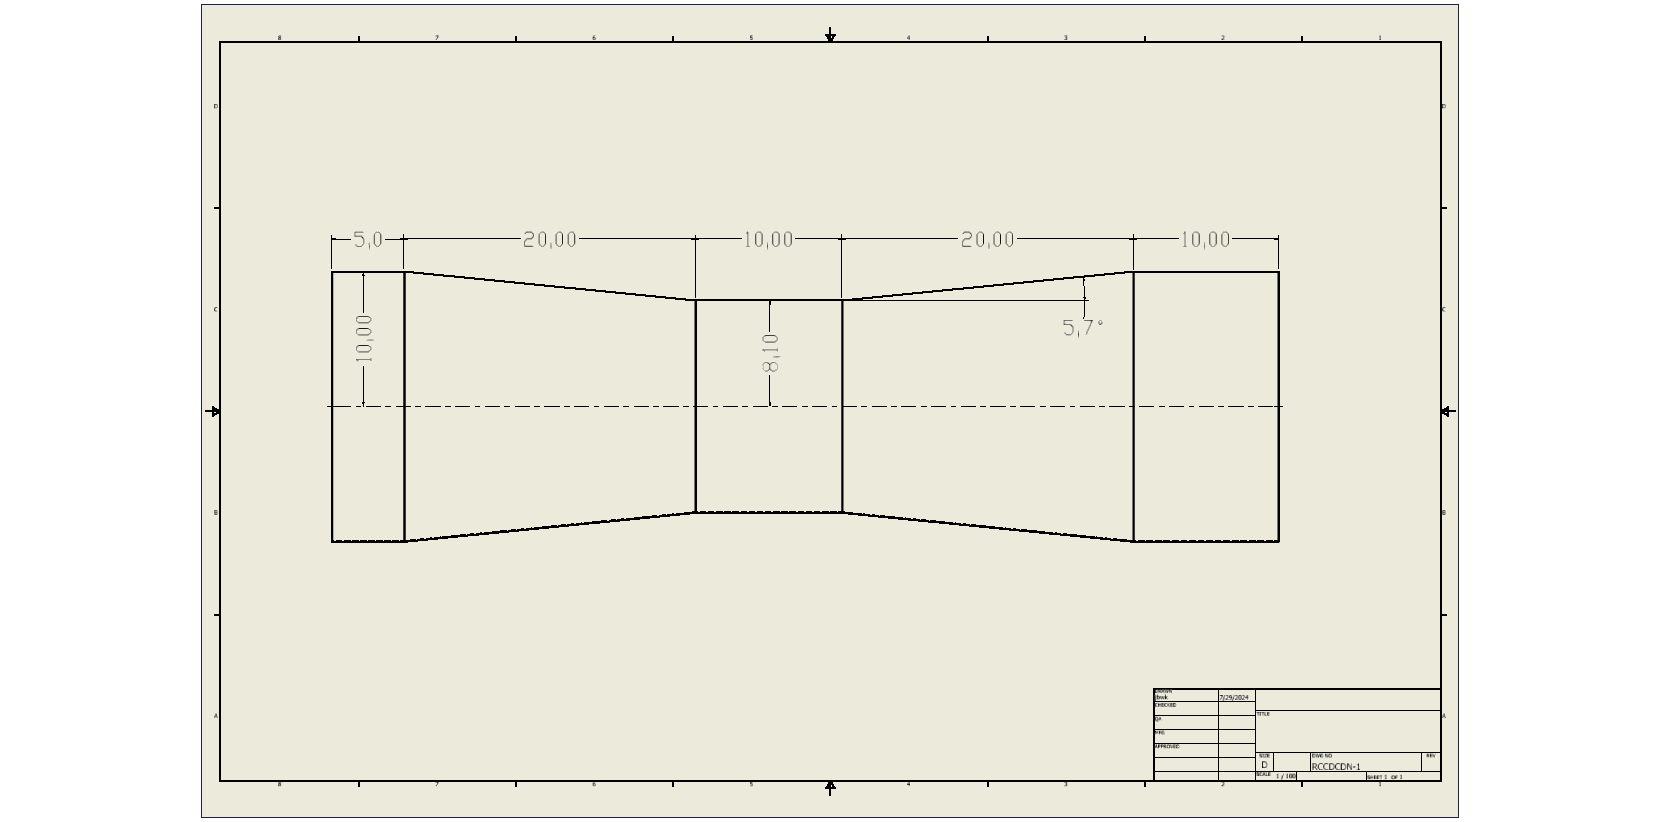
\includegraphics[width=6.80in]{../images/InventortCDNDWG.png}
\captionof{figure}[Dobule Cone]{\textit{Converging-Diverging Nozzel design specifications.}}
\label{fig:InventortCDNDWG}
\end{figure}

%============================================= Image Perf_gan2016 
Fig. \ref{fig:Perf_gan2016}
\begin{multiFigure}
\centering
{
\addFigure{0.40}{../images/Perf_gan2016_01.png} \qquad
\addFigure{0.40}{../imgperm/Perf_gan2016_02.png} \qquad
}
\captionof{figure}[Perfornamce Data Gan]{\textit{Performance plots from \textit{A GPU-based DEM approach for modelling of particulate systems.} \citep{gan2016}.}}
\label{fig:Perf_gan2016}
\end{multiFigure}

%============================================= Image olej 
Fig. \ref{fig:olej}
\begin{figure}[H]
\centering
\includegraphics[width=3.40in]{../images/DoubleCone.png}
\captionof{figure}[Dobule Cone]{\textit{Double-cone Flow field schematic (after Olejniczak,Candler \& Hornung \citep{olejniczak1997}).}}
\label{fig:olej}
\end{figure}

